\chapter{Einleitung}
Bei der Betreuung von Patienten durch einen Therapeuten, ob nun in der Psycho-, Physiotherapie oder sogar in der Diätassistenz, sind neben der eigentlichen \textbf{Therapie / Behandlung} durch den Therapeuten - Übungen und Fragebögen für Zuhause fast immer Bestandteil der Behandlung. Wie in Abbildung \ref{TherapieAblauf} aufgezeigt werden die Aufgaben in der Sitzung besprochen und sollen dann von dem Patienten selbstständig und ohne Betreuung bearbeitet werden.

\begin{figure}[H]
	\centering
	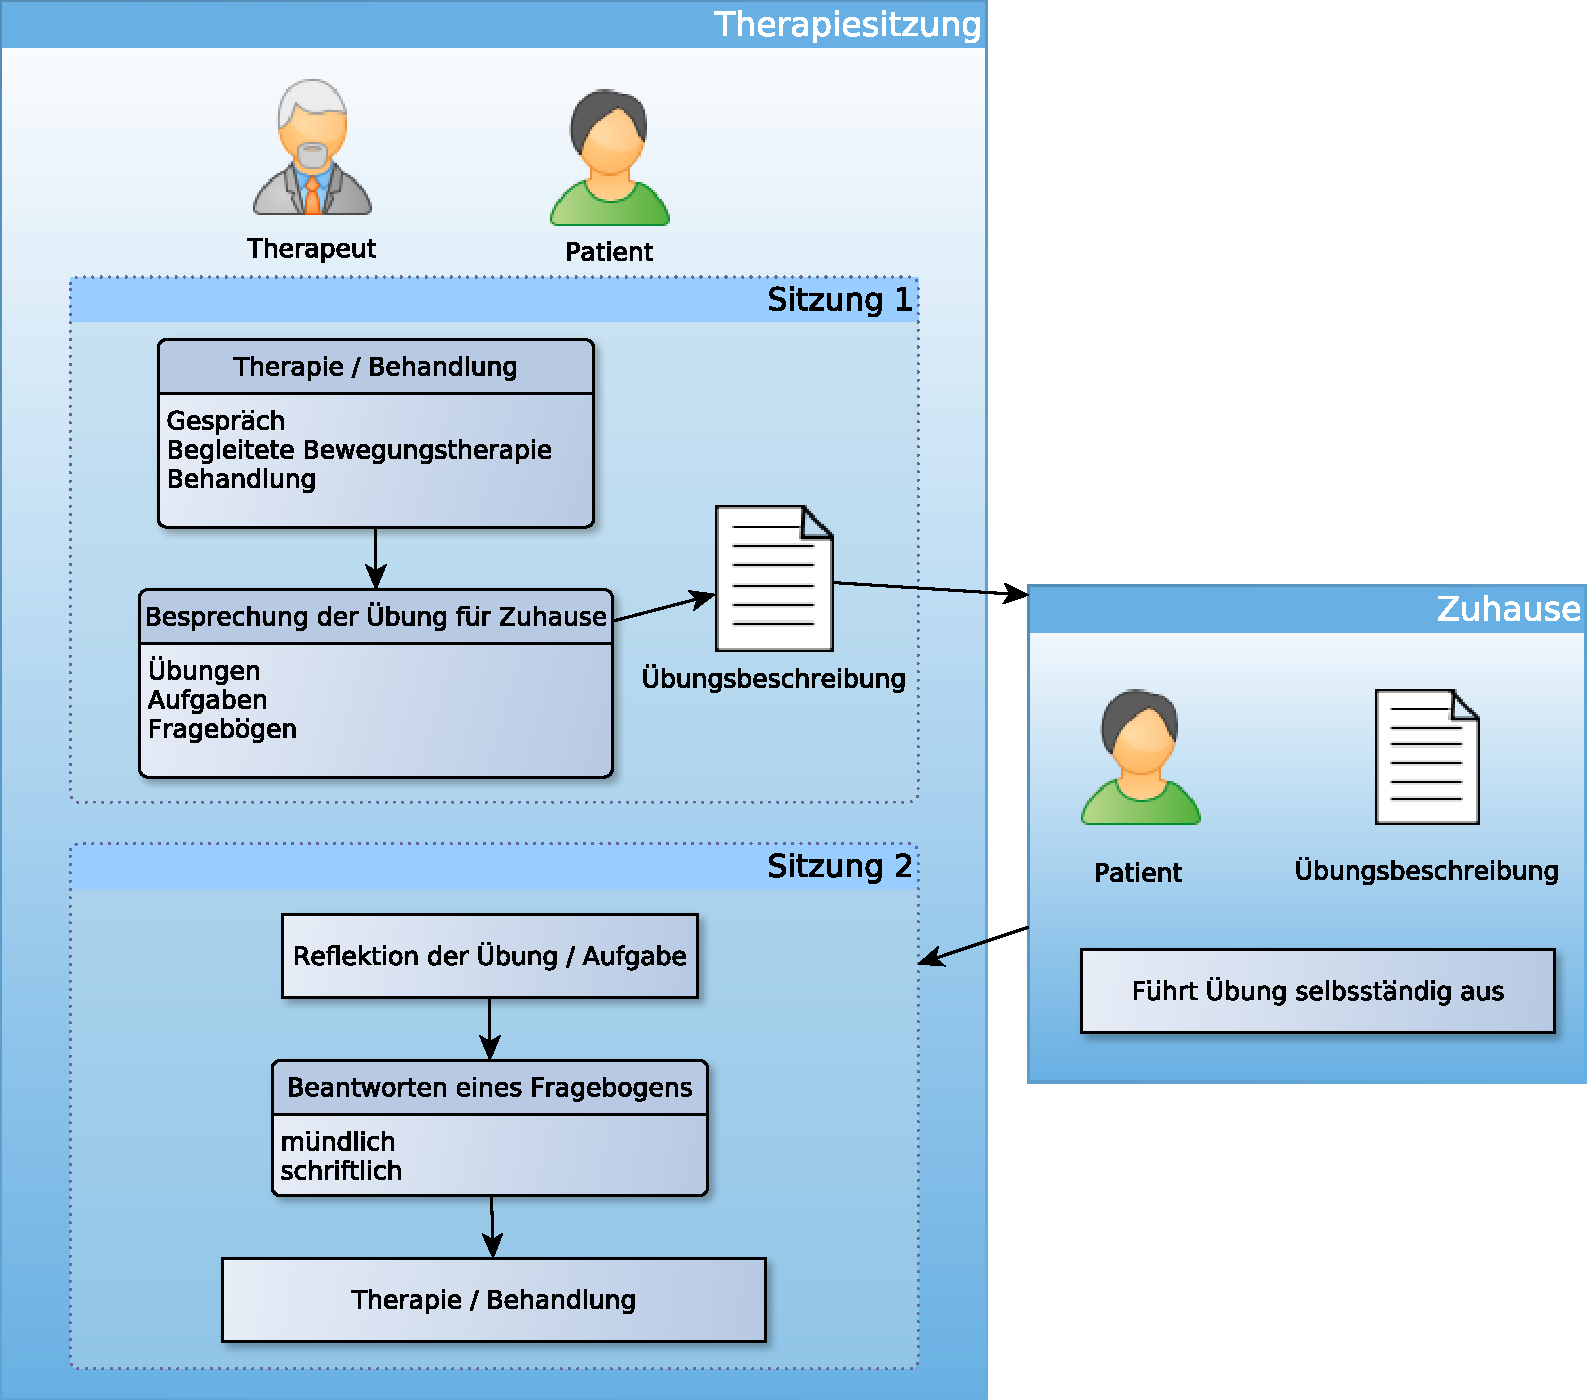
\includegraphics[scale=0.55]{images/TherapieAblauf}
	\caption[Grundlegender Ablauf einer Therapie]{Grundlegender Ablauf einer Therapie}
	\label{TherapieAblauf}
\end{figure}

Diese Aufgaben sind wichtiger Bestandteil für den Behandlungserfolg \cite{SL05}. Sie helfen beim Transfer der Therapie in den Alltag. Jedoch ist eins der größten Probleme bei dieser Vorgehensweise, dass die Aufgaben oft gar nicht oder nur unvollständig erledigt werden \cite{FF01}.

Bisher wurden dieses Aufgaben auf einen Blatt Papier festgehalten und der Patient war selbst dafür verantwortlich diese in seinen Tagesablauf einzuplanen. Die einzige Vorgabe war es, die Aufgabe(n) bis zum nächsten Termin x mal zu machen. Der Therapeut gab im besten Fall lediglich eine Empfehlung wann die Aufgabe zu erledigen ist, nicht jedoch einen genauen Plan an den sich der Patient halten konnte.
\section{Ziel der Arbeit}

Im Zuge dieser Arbeit wurde das Konzept einer Plattform entwickelt und umgesetzt, welches auf der einen Seite dem Patienten hilft sein Aufgabe zu erledigen. Auf der anderen Seite aber auch dem Therapeuten Daten und Feedback zu den Übungen liefert, wodurch dieser die Möglichkeit hat den Behandlungserfolg zu steigern.

Auf Grundlage aktueller Software wurde so eine Plattform implementiert, die es dem Therapeuten erlaubt seine Patienten innerhalb einer Webanwendung zu verwalten. Er hat die Möglichkeit, Therapieaufgaben und Fragebögen zu gestalten und diese dem jeweiligen Patienten zuzuordnen.

Anhand einer App wird der Patient sobald das Zeitintervall angefangen hat, daran erinnert seine Aufgabe zu erledigen und zeigt die Aufgabenbeschreibung an. Am Ende des definierten Zeitintervalls hat der Patient die Möglichkeit den zugeordneten Fragebogen auszufüllen. Welcher nach Beendigung wiederum direkt vom Therapeuten eingesehen werden kann.

Ziel ist es vor allem, das die Aufgaben vollständig und vor allem immer erledigt werden. Aber auch die erzeugte Resonanz und Daten soll zum Therapieerfolg beitragen. Hierdurch können die therapeutischen Aufgaben/Übungen verbessert werden und auf den einzelnen Patienten abgestimmt werden.
\todo{?????????!!!!!!!!!!!!!!}
In einer Studie von Helbig und Fehm \cite{bibid} gaben zwar nur 11\% der Befragten an, die Aufgabe nicht erledigt zu haben. Nicht einmal die Hälfte jedoch gaben dagegen an, die Aufgabe genau so wie beschrieben ausgeführt zu haben. Durch das Anzeigen der Aufgabenbeschreibung soll dem Patienten geholfen werden die Aufgabe genau so durchzuführen wie vorgegeben. Durch die angehängten Materialien in jeglicher digitalen Form kann der Patient vielseitig bei seinem persönlichen Erfolg unterstützt werden.

\section{Aufbau der Arbeit}
\begin{figure}[H]
	\centering
	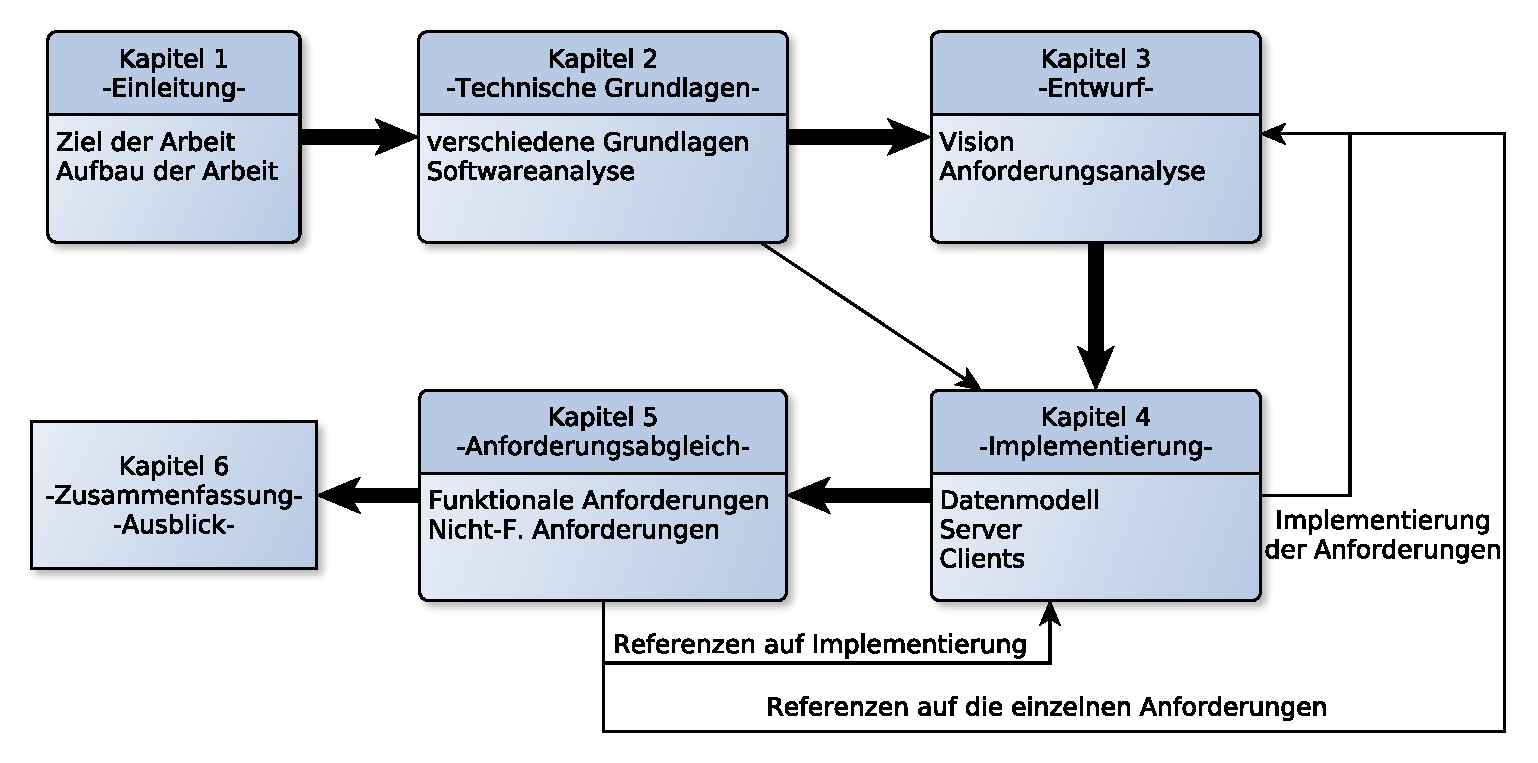
\includegraphics[scale=0.55]{images/AufbauDerArbeit}
	\caption[Aufbau der Arbeit]{Aufbau der Arbeit}
	\label{AufbauDerArbeit}
\end{figure}
Nach dieser Einleitung in das Thema wird im nächsten Kapitel auf die \textbf{technischen Grundlagen} der Arbeit eingegangen. Dieses Kapitel gibt zum einen Grundlagenwissen welches zum besseren Verständnis der Arbeit, insbesondere Kapitel Implementierung, beitragen soll und zum anderen wird eine \textbf{Software/Technologie Analyse} durchgeführt welche sich vorwiegend mit dem Thema Cross-Plattform-Entwicklung für mobile Endgeräte befasst.

Im darauf folgenden Kapitel "< \textbf{Entwurf} "> wird zuerst die \textbf{Vision} der Arbeit vorgestellt, welche darüber Aufschluss gibt, was genau von der entwickelten Plattform erwartet wurde und wie die Mechanismen von statten gehen sollten. Anschließend werden diese Erwartungen im Unterkapitel [\ref{Anforderungsanalyse}] \textbf{Anforderungsanalyse} in \textbf{Anforderungen} umgesetzt. 

In Kapitel \ref{_Implementierung} wird im Detail erklärt auf welche Weise diese \textbf{Anforderungen} umgesetzt sind. Zuerst wird das zugrundeliegende \textbf{Datenmodell} beschrieben. Anschließend werden die \textbf{Implementierungen} von \textbf{Server} und den beiden \textbf{Clients} näher beschrieben.

Im Verlauf von Kapitel \ref{Anforderungsabgleich} werden die \textbf{Anforderungen} aus Kapitel \ref{Anforderungsanalyse} im einzelnen betrachtet und gezeigt ob diese im Laufe der Arbeit erfüllt wurden. Hierbei werden Querverweise zu Kapitel \ref{_Implementierung} hergestellt um es dem Leser einfacher zu machen die zugrundeliegende \textbf{Implementierung} der \textbf{Anforderungen} zu finden.

Im letzten Kapitel wird eine Zusammenfassung sowie ein Ausblick über eine mögliche Weiterführung der Arbeit gegeben.

